%% REPLACE SXXXXXX with your student number
\def\studentNumber{S2617343}


%% START of YOUR ANSWERS
%% Add answers to the questions below, by replacing the text inside the brackets {} for \youranswer{ "Text to be replaced with your answer." }. 
%
% Do not delete the commands for adding figures and tables. Instead fill in the missing values with your experiment results, and replace the images with your own respective figures.
%
% You can generally delete the placeholder text, such as for example the text "Question Figure 2 - Replace the images ..." 
%
% There are 18 TEXT QUESTIONS (a few of the short first ones have their answers added to both the Introduction and the Abstract). Replace the text inside the brackets of the command \youranswer with your answer to the question.
%
% There are also 3 "questions" to replace some placeholder FIGURES with your own, and 3 "questions" asking you to fill in the missing entries in the TABLES provided. 
%
% NOTE! that questions are ordered by the order of appearance of their answers in the text, and not by the order you should tackle them. Specifically, you cannot answer Questions 2, 3, and 4 before concluding all of the relevant experiments and analysis. Similarly, you should fill in the TABLES and FIGURES before discussing the results presented there. 
%
% NOTE! If for some reason you do not manage to produce results for some FIGURES and TABLES, then you can get partial marks by discussing your expectations of the results in the relevant TEXT QUESTIONS (for example Question 8 makes use of Table 1 and Figure 2).
%
% Please refer to the coursework specification for more details.


%% - - - - - - - - - - - - TEXT QUESTIONS - - - - - - - - - - - - 



%% Question 1 - Explain what these figures contain and how the curves evolve, and spot where overfitting occurs. Reason based on the min/max points and velocities (direction and magnitude of change) of the accuracy and error curves
\newcommand{\questionOne} {
\youranswer{the training performance of the model continues to improve, and the curve representing the accuracy remains monotonic on the training set; while the generalization performance of the model becomes very good at the beginning, but after 10 epochs, the generalization performance of the model begins to deteriorate, that is, the model reaches the highest accuracy point on the 10th epoch, and then overfitting occurs, and the gap between training performance and generalization performance becomes larger and larger. Similarly, in Figure~\ref{fig:example_errorcurves}, we can also observe a similar overfitting phenomenon, where the model error decreases on the training set and the validation set, and after the 10th epoch, the model error continues to decrease on the training set, and continues to increase after reaching the lowest point on the validation set}
}

%% Question 2 - Present your network width experiment results by using the relevant figure and table
\newcommand{\questionTwo} {
\youranswer{as the model width increases, the generalization ability of the model will increase, but if the model width is increased indefinitely, overfitting will occur. From Table~\ref{tab:width_exp}, we can see that after the number of neurons in the hidden layer of the model increases from 32 to 64, the performance of the model on the validation set improves, but after the number of neurons increases from 64 to 128, although the performance of the model on the training set becomes better, the performance on the validation set becomes worse. From Figure~\ref{fig:width}, we can see more intuitively that the performance of the model with a width of 32 continues to improve, the model with a width of 64 overfits after the 15th epoch, and the model with a width of 128 overfits after the 10th epoch}   
}

%% Question 3 - Discuss whether varying width affects the results in a consistent way, and whether the results are expected and match well with the prior knowledge (by which we mean your expectations as are formed from the relevant Theory and literature)
\newcommand{\questionThree} {
\youranswer{From the above results, we can see that blindly increasing the model width cannot continuously enhance the generalization ability of the model. Instead, it will cause the model to fall into an overfitting state. This conclusion is consistent with our machine learning theory. When the amount of data remains unchanged, the increase in model capacity will lead to the model's ability to memorize training data during the training process, which may cause the model to begin to capture the noise in the data instead of capturing the essential distribution of the data}
}

%% Question 4 - Present your network depth experiment results by using the relevant figure and table
\newcommand{\questionFour} {
\youranswer{as the depth of the model increases, the generalization ability of the model continues to deteriorate, and overfitting occurs. From Table~\ref{tab:depth_exps}, we can see that as the number of hidden layers of the model increases from 1 to 2 and then to 3, although the performance of the model on the training set improves, the performance on the validation set deteriorates. From Figure~\ref{fig:depth}, we can see more intuitively that all three models enter the overfitting state around the 10th epoch, and the models with 2 and 3 hidden layers overfit faster than the model with only 1 hidden layer}
}

%% Question 5 - Discuss whether varying depth affects the results in a consistent way, and whether the results are expected and match well with the prior knowledge (by which we mean your expectations as are formed from the relevant Theory and literature)
\newcommand{\questionFive} {
\youranswer{Similar to the conclusion of network width, blindly increasing the model depth does not continuously enhance the generalization ability of the model, but instead causes the model to fall into an overfitting state. The increase in model depth leads to an increase in model capacity, which also causes the model to try to memorize training data instead of capturing the essential distribution of the data}
}





%% Question 6 - Explain the experimental details (e.g. hyperparameters), discuss the results in terms of their generalisation performance and overfitting. Select and test the best performing model as part of this analysis.
\newcommand{\questionSix} {
\youranswer{In the experiment of each method, we control the hyperparameters of the baseline unchanged, and only set the hyperparameters of one of the methods (Dropout, L1 Penalty, L2 Penalty, label smoothing). Through multiple experiments, the hyperparameters of the method are observed to affect the model performance while keeping the hyperparameters of other models unchanged. From the results in Table~\ref{tab:hp_search} and Figure~\ref{fig:hp_search}, we can see that as the probability p value of the dropout method decreases, the capacity of the model also decreases, so the generalization performance of the model is alleviated at first, but then it deteriorates and enters the underfitting state in Figure~\ref{fig:dropoutrates}. The L1 penalty performs the same as the dropout in Figure~\ref{fig:weightrates}. As the coefficient of the L2 penalty increases, the generalization effect is worse than the baseline, and the overfitting state is not alleviated. The label smoothing method also alleviates the overfitting state of the baseline. From Table~\ref{tab:hp_search}, we can see that the model with the dropout layer and p set to 0.85 has the best generalization performance, because its validation set error is the lowest at 0.434, and the gap between the validation set and the training set is the smallest}
}

%% Question 7 - Assume you were able to run 8 further training instances (8 specific hyperparameter configurations) where you could combine Dropout and L1, and/or Dropout and L2 regularisation. Which 8 runs would you pick and what question(s) would you aim to answer? Make sure you define the experiment setup, including any relevant hyperparameters
\newcommand{\questionSeven} {
\youranswer{From Table~\ref{tab:hp_search}, we can see that both Dropout and L2 penalty have a certain effect on alleviating overfitting of the baseline. Therefore, we may want to try to combine dropout and L2 penalty in the next experiment to test whether the model can further improve performance. At the same time, we also want to know whether we can choose appropriate hyperparameters for L1 penalty to improve model performance. Therefore, we will set up 8 groups of experiments to try to answer the above questions, where $p$ denotes the probability in Dropout Layer, and $\lambda$ denotes the coefficient in Penalty. For L2 penalty: $(p, \lambda) = \{ (0.85, 5e-4), (0.85, 1e-3), (0.97, 5e-4), (0.97, 1e-3) \}$, for L1 penalty: $(p, \lambda) = \{ (0.85, 1e-4), (0.85, 1e-5), (0.97, 1e-4), (0.97, 1e-5) \}$. At the same time, we keep other model hyperparameters unchanged, such as batchsize of $100$, learning rate of $1e-4$, number of epochs of $100$, the network has $3$ hidden layers, and the number of neurons in each layer is $128$}
}



%% Question 8 - Briefly draw your conclusions based on the results from the previous sections (what are the take-away messages?), discussing them in the context of the overall literature, and conclude your report with a recommendation for future directions
\newcommand{\questionEight} {
\youranswer{In this report, we mainly study the overfitting in machine learning theory through the neural network structure and the setting of regularization methods. By adjusting the width and depth of the neural network, we concluded that increasing the width and depth of the neural network can enhance the generalization performance of the model to a certain extent, but it may also lead to overfitting of the model. Therefore, choosing the right width and depth can achieve high performance while avoiding overfitting. After that, we introduced three regularization methods, namely Dropout, L1/L2 penalty and label smoothing. We conducted experiments on each regularization method and found that adjusting the hyperparameters of these methods can alleviate the overfitting of the model to a certain extent, but choosing the right hyperparameters is necessary. Finally, we also tried to discuss the combination of different regularization methods to see if it can improve the performance of the model. Trying to find the optimal combination configuration and hyperparameters for improving model performance may be a possible research direction in the future, which may be better than using a single regularization method}
}

%% - - - - - - - - - - - - FIGURES - - - - - - - - - - - - 

%% Question Figure 2 - Replace the images in Figure 2 with figures depicting the accuracy and error, training and validation curves for your experiments varying the number of hidden units.
\newcommand{\questionFigureTwo} {
\youranswer{%
\begin{figure}[t]
    \centering
    \begin{subfigure}{\linewidth}
        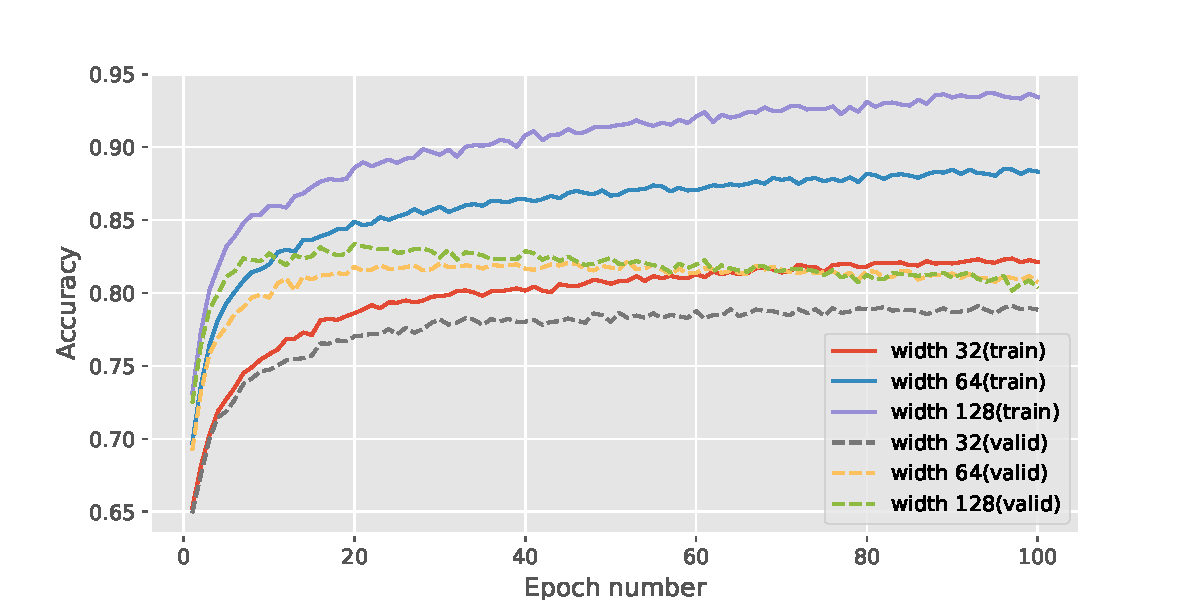
\includegraphics[width=\linewidth]{figures/Task1_acc_curve_width.pdf}
        \caption{accuracy by epoch}
        \label{fig:width_acccurves}
    \end{subfigure} 
    \begin{subfigure}{\linewidth}
        \centering
        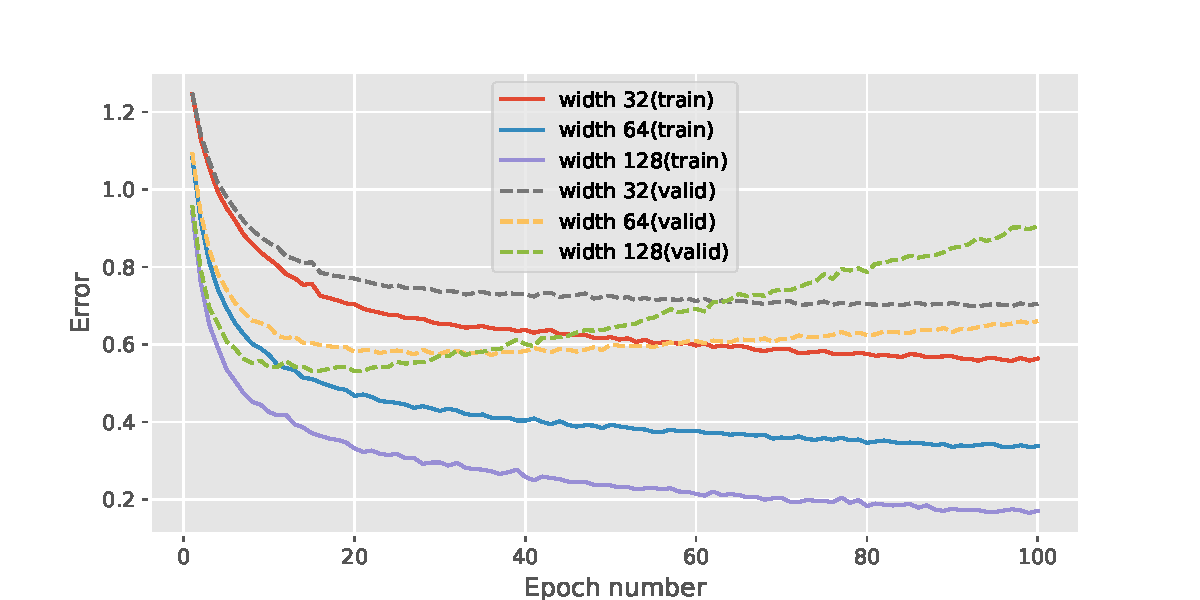
\includegraphics[width=\linewidth]{figures/Task1_error_curve_width.pdf}
        \caption{error by epoch}
        \label{fig:width_errorcurves}
    \end{subfigure} 
    \caption{Training and validation curves in terms of classification accuracy (a) and cross-entropy error (b) on the EMNIST dataset for different network widths.}
    \label{fig:width}
\end{figure} 
}
}

%% Question Figure 3 - Replace these images with figures depicting the accuracy and error, training and validation curves for your experiments varying the number of hidden layers.
\newcommand{\questionFigureThree} {
\youranswer{%
\begin{figure}[t]
    \centering
    \begin{subfigure}{\linewidth}
        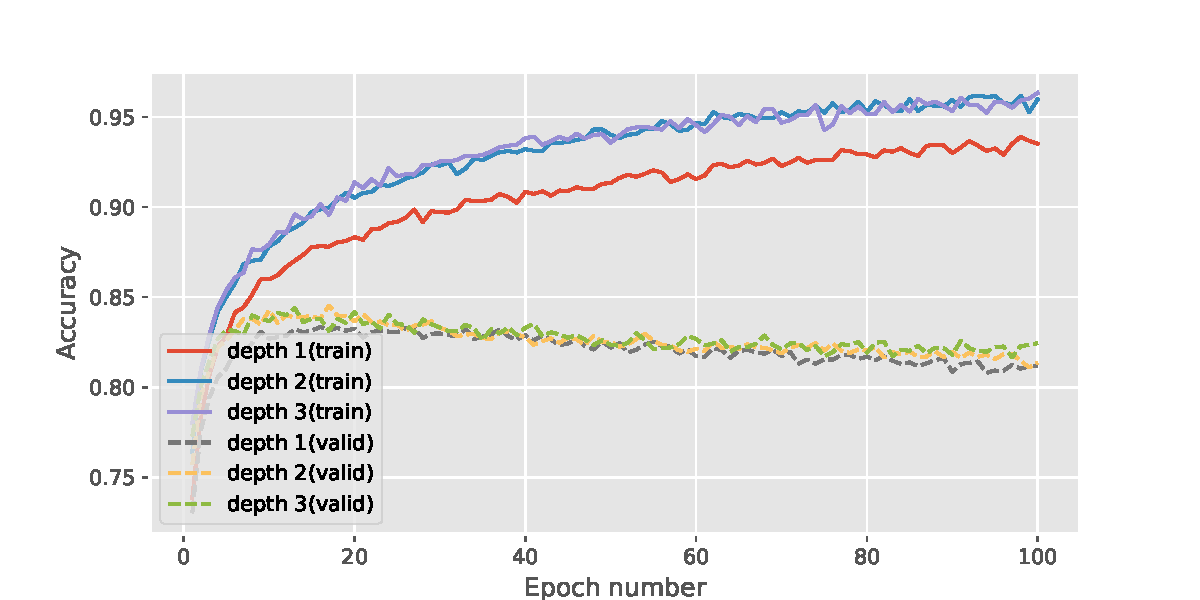
\includegraphics[width=\linewidth]{figures/Task1_acc_curve_depth.pdf}
        \caption{accuracy by epoch}
        \label{fig:depth_acccurves}
    \end{subfigure} 
    \begin{subfigure}{\linewidth}
        \centering
        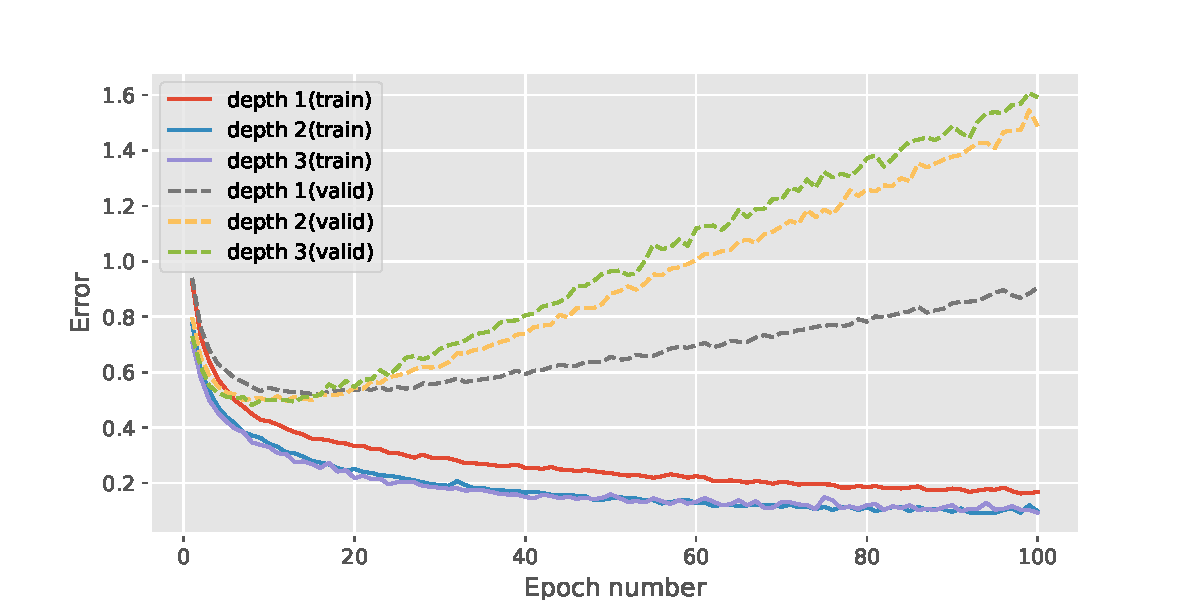
\includegraphics[width=\linewidth]{figures/Task1_error_curve_depth.pdf}
        \caption{error by epoch}
        \label{fig:depth_errorcurves}
    \end{subfigure} 
    \caption{Training and validation curves in terms of classification accuracy (a) and cross-entropy error (b) on the EMNIST dataset for different network depths.}
    \label{fig:depth}
\end{figure} 
}
}

%% Question Figure 4 - Replace these images with figures depicting the Validation Accuracy and Generalisation Gap (difference between validation and training error) for each of the experiment results varying the Dropout inclusion rate, and L1/L2 weight penalty depicted in Table 3 (including any results you have filled in).
\newcommand{\questionFigureFour} {
\youranswer{%
\begin{figure*}[t]
    \centering
    \begin{subfigure}{.475\linewidth}
        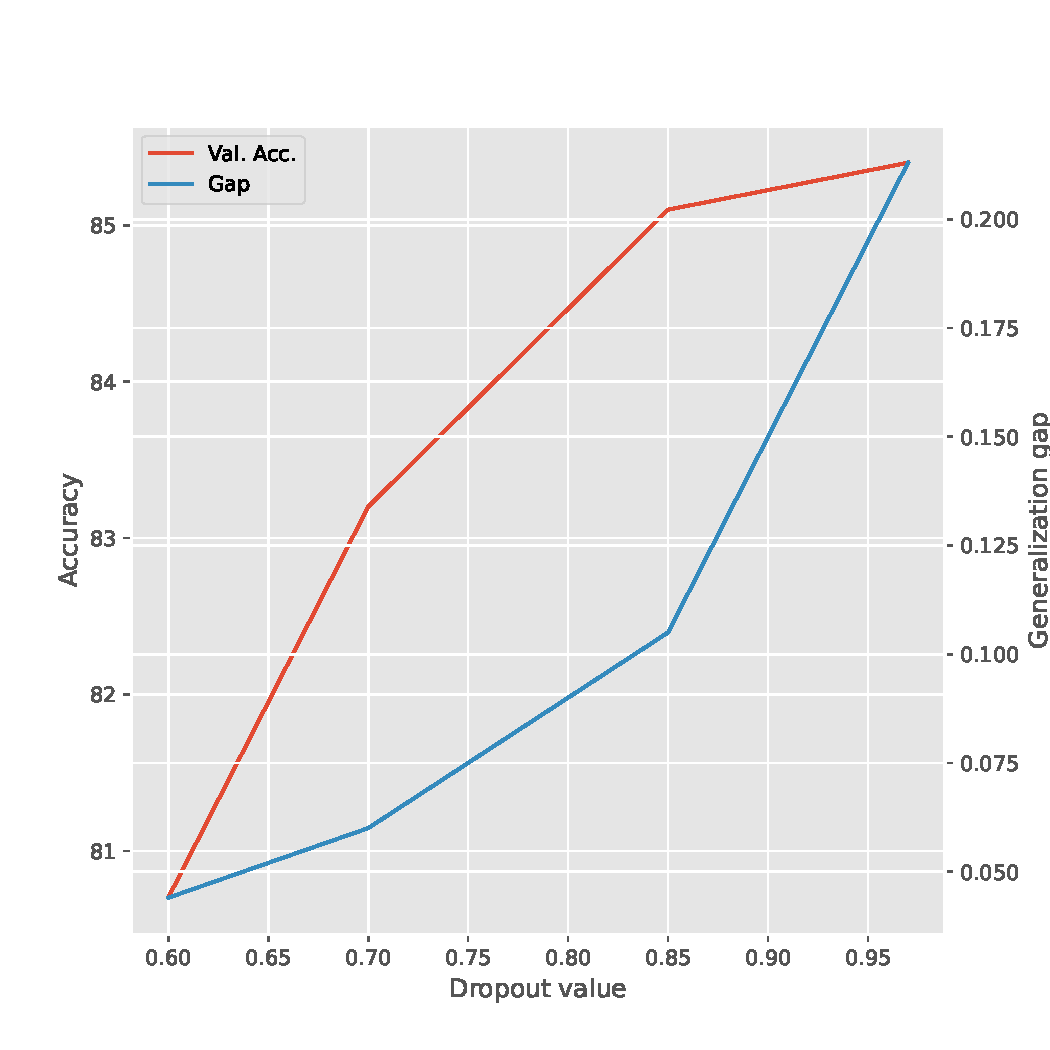
\includegraphics[width=\linewidth]{figures/Task2_dropout_plot.pdf}
        \caption{Accuracy and error by inclusion probability.}
        \label{fig:dropoutrates}
    \end{subfigure} 
    \begin{subfigure}{.475\linewidth}
        \centering
        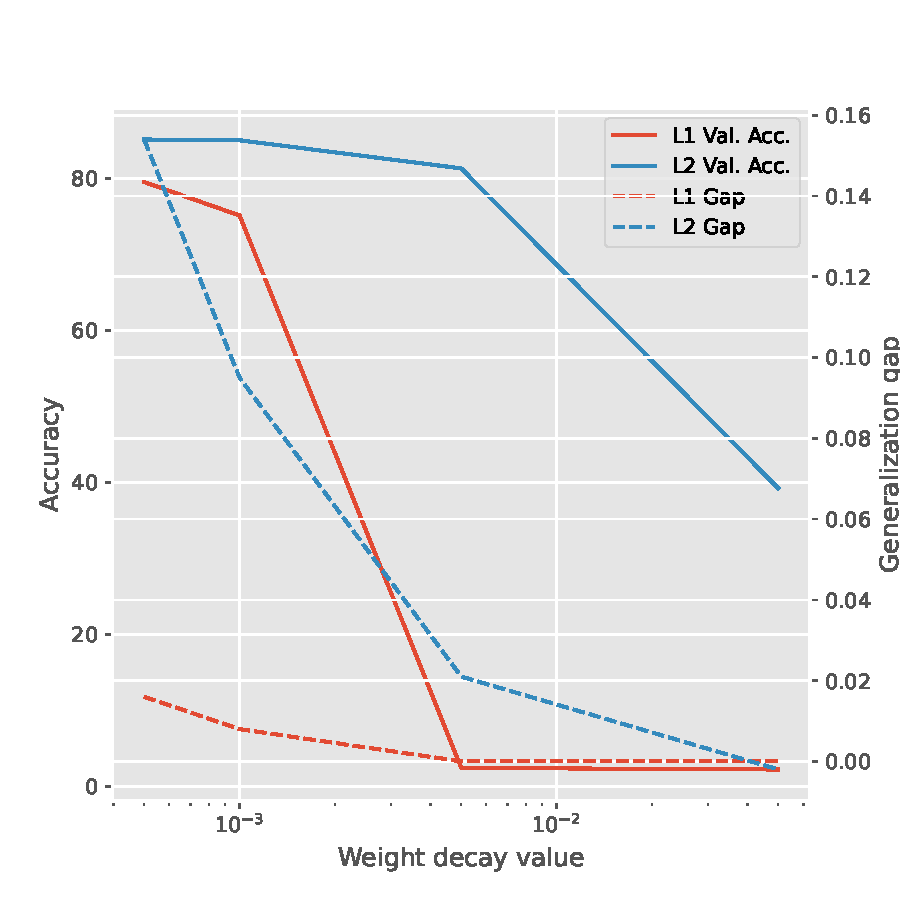
\includegraphics[width=\linewidth]{figures/Task2_wd_plot.pdf}
        \caption{Accuracy and error by weight penalty.}
        \label{fig:weightrates}
    \end{subfigure} 
    \caption{Accuracy and error by regularisation strength of each method (Dropout and L1/L2 Regularisation).}
    \label{fig:hp_search}
\end{figure*}
}
}

%% - - - - - - - - - - - - TABLES - - - - - - - - - - - - 

%% Question Table 1 - Fill in Table 1 with the results from your experiments varying the number of hidden units.
\newcommand{\questionTableOne} {
\youranswer{
\begin{table}[t]
    \centering
    \begin{tabular}{c|ccc}
    \toprule
        \# Hidden Units & Val. Acc. & Train Error & Val. Error\\
    \midrule
         32            &    78.9   &  0.563 &   0.705            \\
         64            &    80.8   &  0.337  &   0.660               \\
         128           &    80.4   &  0.17  &   0.907           \\ 
    \bottomrule
    \end{tabular}
    \caption{Validation accuracy (\%) and training/validation error (in terms of cross-entropy error) for varying network widths on the EMNIST dataset.}
    \label{tab:width_exp}
\end{table}
}
}

%% Question Table 2 - Fill in Table 2 with the results from your experiments varying the number of hidden layers.
\newcommand{\questionTableTwo} {
\youranswer{\begin{table}[t]
    \centering
    \begin{tabular}{c|ccc}
    \toprule
        \# Hidden Layers & Val. Acc. & Train Error & Val. Error \\
    \midrule
         1               &      81.2      &   0.168 & 0.905                \\
         2               &      81.4      &   0.098 & 1.488                \\
         3               &      82.4      &   0.093 & 1.592                \\ 
    \bottomrule
    \end{tabular}
    \caption{Validation accuracy (\%) and training/validation error (in terms of cross-entropy error) for varying network depths on the EMNIST dataset.}
    \label{tab:depth_exps}
\end{table}
}
}

%% Question Table 3 - Fill in Table 3 with the results from your experiments for the missing hyperparameter values for each of L1 regularisation, L2 regularisation, Dropout and label smoothing (use the values shown on the table).
\newcommand{\questionTableThree} {
\youranswer{\begin{table*}[t]
    \centering
    \begin{tabular}{c|c|ccc}
    \toprule
        Model    &  Hyperparameter value(s) & Validation accuracy & Train Error & Validation Error \\
    \midrule
    \midrule
        Baseline &  -                    &               0.837 &       0.241 &  0.533          \\
    \midrule
        \multirow{4}*{Dropout}
                 & 0.6                   &  80.7                &      0.549 & 0.593     \\
                 & 0.7 & 83.2 & 0.444 & 0.504  \\
                 & 0.85 & 85.1 &  0.329 &  \textbf{\textit{0.434}} \\
                 & 0.97 & \textbf{\textit{85.4}} &  \textbf{\textit{0.244}} & 0.457  \\
    \midrule
        \multirow{4}*{L1 penalty}
                 & 5e-4 & \textit{79.5} & \textit{0.642} & \textit{0.658} \\
                 & 1e-3 & 75.1 & 0.841 & 0.849 \\
                 & 5e-3 & 2.41 & 3.850 & 3.850 \\
                 & 5e-2 & 2.20 & 3.850 & 3.850 \\
    \midrule
        \multirow{4}*{L2 penalty}  
                 & 5e-4 & \textit{85.1} & \textit{0.306} & 0.460 \\
                 & 1e-3 & 85.0 & 0.361 & \textit{0.456} \\
                 & 5e-3 & 81.3 & 0.586 & 0.607 \\
                 & 5e-2 & 39.2 & 2.258 & 2.256  \\
    \midrule
        Label smoothing & 0.1 & 85.4 & 1.017 & 1.152 \\
    \bottomrule
    \end{tabular}
    \caption{Results of all hyperparameter search experiments. \emph{italics} indicate the best results per series (Dropout, L1 Regularisation, L2 Regularisation, Label smoothing) and \textbf{bold} indicates the best overall.}
    \label{tab:hp_search}
\end{table*}
}
}

%% END of YOUR ANSWERS